% !TeX root = main.tex

Los Merkle Trees son estructuras de datos basadas en árboles binarios y funciones de hash criptográficas que se utilizan extensivamente como parte de protocolos criptográficos en el ROM.

\begin{definition}[Merkle Tree]
	Sea $L = \{\ell_1, \ldots, \ell_n\} \subset \{0,1\}^*$ un conjunto de datos, y sea $\mathcal{H}: \{0,1\}^* \to \{0,1\}^m$ una función de hash criptográfica. Un Merkle Tree es un árbol binario $\mathcal{T}_{L,\mathcal{H}}$ (notado $\mathcal{T}$ por comodidad) sobre el conjunto de datos $D$, definido recursivamente de la siguiente manera:
	\begin{enumerate}
		\item En el nivel inferior, están las hojas del árbol, que son los hashes de los datos ordenados: $h_i = \mathcal{H}(\ell_i)$, para $1 \leq i \leq n$.
		\item Cada nodo interno $N$ con hijos $N_i$ (nodo hijo izquierdo) y $N_d$ (nodo hijo derecho) se define como $N = \mathcal{H}(N_i \Vert N_d)$, donde $\Vert$ denota la operación de concatenación en $\{0,1\}^*$.
		\item Se le llama Merkle Root de $\mathcal{T}$, notada $r(\mathcal{T})$, a la raíz del árbol. Es el nodo que sintetiza criptográficamente toda la información de $L$.
	\end{enumerate}
	 En caso de que el número de hojas no sea una potencia de 2, se puede duplicar la última hoja o aplicar otra estrategia de padding para completar un árbol binario completo.
\end{definition}

La propiedad clave de un Merkle Tree $r(\mathcal{T})$ es que cualquier modificación en un dato $\ell_i$ provoca un cambio en su hoja asociada $\mathcal{H}(\ell_i)$, y se propaga hasta $r(\mathcal{T})$ de una forma impredecible. Esto permite verificar la integridad de un elemento específico sin necesidad de recorrer o almacenar todo el conjunto de datos. Cualquier modificación en un dato (incluso en un solo bit) permite detectar alteraciones de forma inmediata solamente verificando el valor de $r(\mathcal{T})$.

Por supuesto, el conjunto de datos puede pertenecer a cualquier conjunto arbitrario $X$ mientras todos sus datos sean finitos, y transformarlos a tiras de bits, replicando lo que hicimos en la sección anterior.

Observar que en las imágenes se indica el conjunto de datos por debajo de $\mathcal{T}$, pero se recalca que estos no pertenecen directamente a $\mathcal{T}$, sino que el nivel inferior de $\mathcal{T}$ está compuesto por los $\mathcal{H}(\ell_i)$.

\begin{figure}[h]
	\centering
	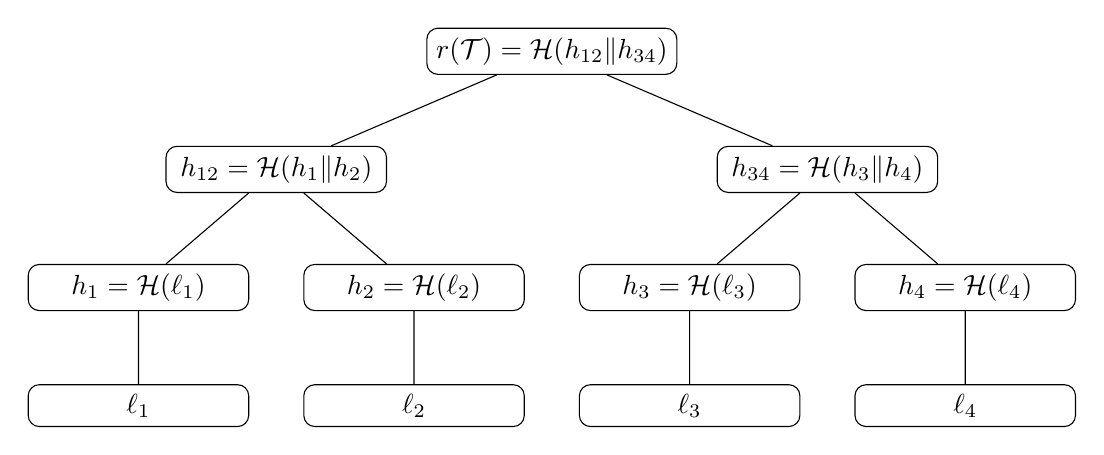
\begin{tikzpicture}[
		level 1/.style={level distance=1.5cm, sibling distance=7cm},
		level 2/.style={level distance=1.5cm, sibling distance=3.5cm},
		level 3/.style={level distance=1.5cm, sibling distance=2cm},
		every node/.style={
			draw,
			rectangle,
			rounded corners,
			align=center,
			minimum width=2.8cm
		}
		]
		
		\node {$r(\mathcal{T}) = \mathcal{H}(h_{12} \Vert h_{34})$}
		child {
			node {$h_{12} = \mathcal{H}(h_1 \Vert h_2)$}
			child {
				node {$h_1 = \mathcal{H}(\ell_1)$}
				child { node {$\ell_1$} }
			}
			child {
				node {$h_2 = \mathcal{H}(\ell_2)$}
				child { node {$\ell_2$} }
			}
		}
		child {
			node {$h_{34} = \mathcal{H}(h_3 \Vert h_4)$}
			child {
				node {$h_3 = \mathcal{H}(\ell_3)$}
				child { node {$\ell_3$} }
			}
			child {
				node {$h_4 = \mathcal{H}(\ell_4)$}
				child { node {$\ell_4$} }
			}
		};
		
	\end{tikzpicture}
	\caption{Merkle Tree tradicional}
	\label{fig:classic-merkle-tree}
\end{figure}

Otra cosa importantísima que nos permite hacer esta estructura son pruebas de pertenencia, también conocidas como Merkle Proofs. Esta es la primera introducción a las pruebas que vamos a tener en el desarrollo de esta tesis. Una Merkle Proof permite demostrar que un elemento pertenece a un Merkle Tree $\mathcal{T}$ sin necesidad de revelar todos los elementos del conjunto de datos asociado, lo que es útil para no tener que almacenar la totalidad de $\mathcal{T}$ para verificar un solo dato, sino solamente $r(\mathcal{T})$. En algún lugar se tiene que guardar $\mathcal{T}$, pero hace innecesario replicarlo en más lugares.

\begin{definition}[Merkle Proof]
	Sea $\mathcal{T}$ un Merkle Tree con raíz $r(\mathcal{T})$, construido sobre un conjunto de datos $L = \{\ell_1, \ldots, \ell_n\}$ y usando una función de hash criptográfica $\mathcal{H}$. Una Merkle Proof para un dato $\ell \in L$ es una lista ordenada $\pi = [(h_1, b_1), \ldots, (h_k, b_k)]$ que representa un camino (Merkle Path) desde la hoja correspondiente a $\ell$ hasta $r(\mathcal{T})$, donde:
	\begin{itemize}
		\item Cada $h_i \in \{0,1\}^n$ es el hash del hermano del nodo del nivel $i$ en el camino desde la hoja correspondiente a $\ell$ hasta $r(\mathcal{T})$.
		\item Cada $b_i \in \{0,1\}$ es un bit que indica si el hash $h_i$ está a la izquierda ($b_i = 0$) o a la derecha ($b_i = 1$) del nodo en el camino.
		\item $k = \lfloor \log_2 n \rfloor$ es la altura de $\mathcal{T}$, por lo tanto la cantidad de pasos en el camino hasta $r(\mathcal{T})$.
	\end{itemize}
\end{definition}

\begin{figure}[h]
	\centering
	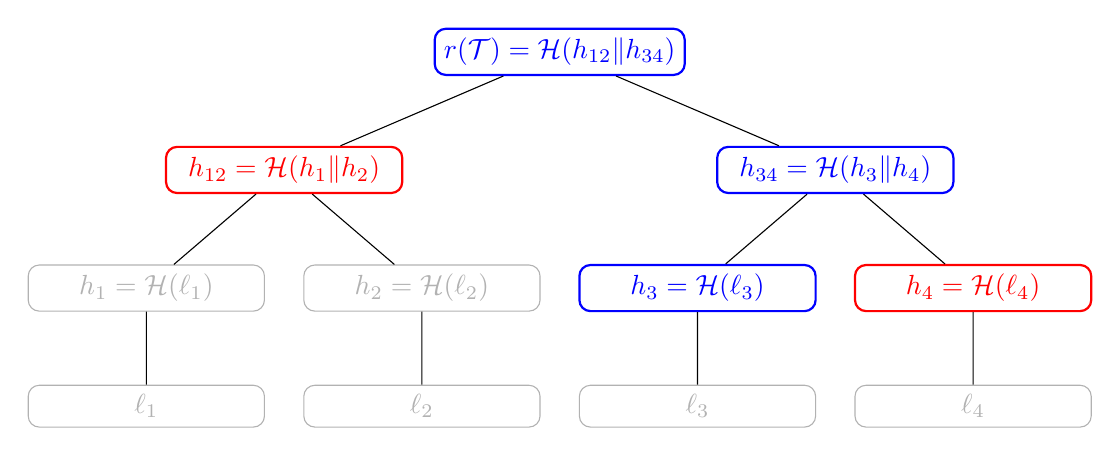
\begin{tikzpicture}[
		level 1/.style={level distance=1.5cm, sibling distance=7cm},
		level 2/.style={level distance=1.5cm, sibling distance=3.5cm},
		level 3/.style={level distance=1.5cm, sibling distance=2cm},
		proof/.style={
			draw, thick, red, rectangle, rounded corners, align=center, minimum width=3cm
		},
		pathnode/.style={
			draw, thick, blue, rectangle, rounded corners, align=center, minimum width=3cm
		},
		normal/.style={
			draw, rectangle, rounded corners, align=center, minimum width=3cm, opacity=0.3
		}
		]
		
		\node[pathnode] {$r(\mathcal{T}) = \mathcal{H}(h_{12} \Vert h_{34})$}
		child {
			node[proof] {$h_{12} = \mathcal{H}(h_1 \Vert h_2)$}  % resaltado en rojo, parte de la proof
			child {
				node[normal] {$h_1 = \mathcal{H}(\ell_1)$}
				child { node[normal] {$\ell_1$} }
			}
			child {
				node[normal] {$h_2 = \mathcal{H}(\ell_2)$}
				child { node[normal] {$\ell_2$} }
			}
		}
		child {
			node[pathnode] {$h_{34} = \mathcal{H}(h_3 \Vert h_4)$}  % nodo intermedio azul, parte del camino
			child {
				node[pathnode] {$h_3 = \mathcal{H}(\ell_3)$}          % hoja azul, camino a la raíz
				child { node[normal] {$\ell_3$} }
			}
			child {
				node[proof] {$h_4 = \mathcal{H}(\ell_4)$}           % resaltado en rojo, parte de la proof
				child { node[normal] {$\ell_4$} }
			}
		};
	\end{tikzpicture}
	\caption{Merkle Proof de pertenencia de $\ell_3$ en $L$}
	\label{fig:verify-merkle-proof}
\end{figure}

En la imagen de una Merkle Proof, se observa que es una prueba de pertenencia de $\ell_3$, y que $\pi = [h_4, h_{12}]$. Se puede definir una función (y su algoritmo correspondiente) para verificar que una Merkle Proof es correcta. La idea es reconstruir determinísticamente los nodos del Merkle Path del dato en $\mathcal{T}$ (en azul en la figura \ref{fig:verify-merkle-proof}) usando $\pi$ (en rojo en la figura \ref{fig:verify-merkle-proof}) para llegar hasta $r(\mathcal{T})$, y verificar que es igual al valor esperado. Los bits $b_i$ son esenciales para preservar el orden de concatenación dentro del input de $\mathcal{H}$. Este método es seguro, en tanto $\mathcal{H}$ es una función de hash criptográfica, y por lo tanto es resistente a colisiones.

\begin{definition}[Función de verificación de Merkle Proof]
	Sea $\mathcal{T}$ un Merkle Tree con raíz $r(\mathcal{T})$, construido usando una función de hash criptográfica $\mathcal{H}$, y sea $\pi$ una Merkle Proof para un dato $l \in L$. Definimos la función de verificación de $\pi$ como:
	$$\mathsf{Verify}(\ell, \pi, r(\mathcal{T})) = \llbracket x_k = r(\mathcal{T}) \rrbracket,$$
	donde
	$$x_0 := \mathcal{H}(\ell), \qquad x_i := \begin{cases}
		\mathcal{H}(h_i \Vert x_{i-1}) & \text{si } b_i = 0, \\
		\mathcal{H}(x_{i-1} \Vert h_i) & \text{si } b_i = 1,
	\end{cases} \quad 1 \leq i \leq k.$$
\end{definition}

\begin{algorithm}[h]
	\caption{Verificación de una Merkle Proof}
	\label{alg:verify-merkle-proof}
	\begin{algorithmic}[1]
		\Require Dato $\ell \in \{0,1\}^*$, Merkle Proof $\pi = [(h_1,b_1), \ldots, (h_k,b_k)]$, raíz $r(\mathcal{T}) \in \{0,1\}^n$
		\Ensure \textbf{true} si $\pi$ prueba que $\ell \in \mathcal{T}$, \textbf{false} en caso contrario
		\State $x \gets \mathcal{H}(\ell)$
		\For{$i = 1$ \textbf{to} $k$}
		\If{$b_i = 0$} \Comment{$h_i$ es hijo izquierdo}
		\State $x \gets \mathcal{H}(h_i \Vert x)$
		\Else \Comment{$h_i$ es hijo derecho}
		\State $x \gets \mathcal{H}(x \Vert h_i)$
		\EndIf
		\EndFor
		\State \Return $\llbracket x = r(\mathcal{T}) \rrbracket$
	\end{algorithmic}
\end{algorithm}

Notar que el algoritmo \ref{alg:verify-merkle-proof} tiene una complejidad temporal de $O(k) = O(\log n)$, así como el tamaño de la Merkle Proof. Para árboles con muchos niveles, esto resulta clave.

TODO: Batch Merkle Proof (OPCIONAL depende como salga reunion con Mithril)



